% Options for packages loaded elsewhere
\PassOptionsToPackage{unicode}{hyperref}
\PassOptionsToPackage{hyphens}{url}
%
\documentclass[
]{book}
\usepackage{lmodern}
\usepackage{amssymb,amsmath}
\usepackage{ifxetex,ifluatex}
\ifnum 0\ifxetex 1\fi\ifluatex 1\fi=0 % if pdftex
  \usepackage[T1]{fontenc}
  \usepackage[utf8]{inputenc}
  \usepackage{textcomp} % provide euro and other symbols
\else % if luatex or xetex
  \usepackage{unicode-math}
  \defaultfontfeatures{Scale=MatchLowercase}
  \defaultfontfeatures[\rmfamily]{Ligatures=TeX,Scale=1}
\fi
% Use upquote if available, for straight quotes in verbatim environments
\IfFileExists{upquote.sty}{\usepackage{upquote}}{}
\IfFileExists{microtype.sty}{% use microtype if available
  \usepackage[]{microtype}
  \UseMicrotypeSet[protrusion]{basicmath} % disable protrusion for tt fonts
}{}
\makeatletter
\@ifundefined{KOMAClassName}{% if non-KOMA class
  \IfFileExists{parskip.sty}{%
    \usepackage{parskip}
  }{% else
    \setlength{\parindent}{0pt}
    \setlength{\parskip}{6pt plus 2pt minus 1pt}}
}{% if KOMA class
  \KOMAoptions{parskip=half}}
\makeatother
\usepackage{xcolor}
\IfFileExists{xurl.sty}{\usepackage{xurl}}{} % add URL line breaks if available
\IfFileExists{bookmark.sty}{\usepackage{bookmark}}{\usepackage{hyperref}}
\hypersetup{
  pdftitle={O czym śpiewają Holendrzy?},
  pdfauthor={Jacek Pardyak},
  hidelinks,
  pdfcreator={LaTeX via pandoc}}
\urlstyle{same} % disable monospaced font for URLs
\usepackage{longtable,booktabs}
% Correct order of tables after \paragraph or \subparagraph
\usepackage{etoolbox}
\makeatletter
\patchcmd\longtable{\par}{\if@noskipsec\mbox{}\fi\par}{}{}
\makeatother
% Allow footnotes in longtable head/foot
\IfFileExists{footnotehyper.sty}{\usepackage{footnotehyper}}{\usepackage{footnote}}
\makesavenoteenv{longtable}
\usepackage{graphicx}
\makeatletter
\def\maxwidth{\ifdim\Gin@nat@width>\linewidth\linewidth\else\Gin@nat@width\fi}
\def\maxheight{\ifdim\Gin@nat@height>\textheight\textheight\else\Gin@nat@height\fi}
\makeatother
% Scale images if necessary, so that they will not overflow the page
% margins by default, and it is still possible to overwrite the defaults
% using explicit options in \includegraphics[width, height, ...]{}
\setkeys{Gin}{width=\maxwidth,height=\maxheight,keepaspectratio}
% Set default figure placement to htbp
\makeatletter
\def\fps@figure{htbp}
\makeatother
\setlength{\emergencystretch}{3em} % prevent overfull lines
\providecommand{\tightlist}{%
  \setlength{\itemsep}{0pt}\setlength{\parskip}{0pt}}
\setcounter{secnumdepth}{5}
% new for polish
\usepackage{polski}
\usepackage[polish]{babel}
%\usepackage[utf8]{inputenc}

% ------------
\usepackage{booktabs}
\usepackage{amsthm}
\makeatletter
\def\thm@space@setup{%
  \thm@preskip=8pt plus 2pt minus 4pt
  \thm@postskip=\thm@preskip
}
% ------------
% new for columns
\newenvironment{columns}[1][]{}{}

\newenvironment{column}[1]{\begin{minipage}{#1}\ignorespaces}{%
\end{minipage}
\ifhmode\unskip\fi
\aftergroup\useignorespacesandallpars}

\def\useignorespacesandallpars#1\ignorespaces\fi{%
#1\fi\ignorespacesandallpars}

\makeatletter
\def\ignorespacesandallpars{%
  \@ifnextchar\par
    {\expandafter\ignorespacesandallpars\@gobble}%
    {}%
}
\makeatother
\usepackage[]{natbib}
\bibliographystyle{apalike}

\title{O czym śpiewają Holendrzy?}
\author{Jacek Pardyak}
\date{2020-04-27}

\begin{document}
\maketitle

{
\setcounter{tocdepth}{1}
\tableofcontents
}
\hypertarget{wstux119p}{%
\chapter{Wstęp}\label{wstux119p}}

Wszelkie prawa do tekstów piosenek umieszczonych w tej pracy przysługują ich autorom.

Teksty piosenek znajdują się tutaj wyłącznie w celach informacyjnych i edukacyjnych oraz służą do użytku prywatnego.

W przypadku, gdy właściciel praw do konkretnego tekstu nie życzy sobie by się nim posługiwać w tej pracy, uprzejmie proszę o kontakt, a tekst zostanie usunięty.

Wszelkie prawa do tłumaczeń tekstów piosenek umieszczonych w tej pracy przysługują mi, ich autorowi.

\hypertarget{top-2000}{%
\chapter{TOP 2000}\label{top-2000}}

\hypertarget{Leef}{%
\section{\texorpdfstring{Leef, \emph{André Hazes jr.}}{Leef, André Hazes jr.}}\label{Leef}}

\begin{column}{0.33\textwidth}

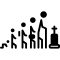
\includegraphics{./images/Leef}

\end{column}

\begin{column}{0.34\textwidth}

~

\end{column}

\begin{column}{0.33\textwidth}

\textbf{Leef} \citep{Leef} {[}\emph{Żyj}{]} to piosenka o życiu i umieraniu. Rozpoczyna się w scenerii podobnej do tej z piosenki \ref{Een-beetje-verliefd} wykonanej przez ojca André Hazes.

\end{column}

\vfill

\begin{column}{0.48\textwidth}

Op een vrijdag in de kroeg ergens in Amsterdam\\
Zat aan de bar met een glas een oude wijze man\\
Hij zei dat die nog maar een paar dagen had\\
Dus pak het leven, pak alles en ga er mee op pad

\end{column}

\begin{column}{0.04\textwidth}

~

\end{column}

\begin{column}{0.48\textwidth}

W piątek w pubie w Amsterdamie siedział\\
Stary mądry człowiek ze szklanką przy barze\\
Powiedział, że zostało mu jeszcze tylko kilka dni\\
Więc chwytaj życie, weź wszystko i ruszaj ze mną

\end{column}

\vfill

\begin{column}{0.48\textwidth}

\emph{En hij zei: '\,'Leef, alsof het je laatste dag is}\\
\emph{Leef, alsof de morgen niet bestaat}\\
\emph{Leef, alsof het nooit echt af is}\\
\emph{En leef, pak alles wat je kan'\,'}

\end{column}

\begin{column}{0.04\textwidth}

~

\end{column}

\begin{column}{0.48\textwidth}

\emph{I rzekł: '\,'Żyj, jakby to był twój ostatni dzień}\\
\emph{Żyj, jakby nie miało być jutra}\\
\emph{Żyj, jakby to nie był koniec do końca}\\
\emph{I żyj, łap wszystko'\,'}

\end{column}

\vfill

\begin{column}{0.48\textwidth}

\emph{En ga, a, a, a}\\
\emph{A, a, a, a}\\
\emph{A, a, a, a}\\
\emph{Pak alles wat je kan}

\end{column}

\begin{column}{0.04\textwidth}

~

\end{column}

\begin{column}{0.48\textwidth}

\emph{I leć, a, a, a}\\
\emph{A, a, a, a}\\
\emph{A, a, a, a}\\
\emph{Łap wszystko, co możesz}

\end{column}

\vfill

\begin{column}{0.48\textwidth}

\emph{En ga, a, a, a}\\
\emph{A, a, a, a}\\
\emph{Ga}\\
\emph{Pak alles wat je kan}

\end{column}

\begin{column}{0.04\textwidth}

~

\end{column}

\begin{column}{0.48\textwidth}

\emph{I leć, a, a, a}\\
\emph{A, a, a, a}\\
\emph{Leć}\\
\emph{Łap wszystko, co możesz}

\end{column}

\vfill

\begin{column}{0.48\textwidth}

Hij vertelde dat 'ie zich had gewerkt in het zweet\\
Geld verdiend als water maar nooit echt had geleefd\\
Z'n vrouw was bij hem weg, voor een ander ingeruild\\
Af en toe gelachen maar veel te veel gehuild

\end{column}

\begin{column}{0.04\textwidth}

~

\end{column}

\begin{column}{0.48\textwidth}

Opowiedział, jak się w życiu napocił przy robocie\\
Pieniądze spływały lekko ale nigdy nie żył naprawdę\\
Żona go opuściła zamieniła sobie na innego\\
Zbyt mało śmiał się a zbyt dużo się napłakał

\end{column}

\vfill

\begin{quote}
\textbf{Hij is zo vlug als water.} On chwyta w biegu.\\
\textbf{Ik wilde net op pad gaan.} Właśnie miałem wyruszyć w drogę.\\
\textbf{Gele gans zelf.} Zażółć gęślą jaźń.
\end{quote}

\hypertarget{Een-beetje-verliefd}{%
\section{\texorpdfstring{Een beetje verliefd, \emph{André Hazes}}{Een beetje verliefd, André Hazes}}\label{Een-beetje-verliefd}}

\begin{column}{0.33\textwidth}

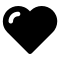
\includegraphics{./images/Een-beetje-verliefd}

\end{column}

\begin{column}{0.34\textwidth}

~

\end{column}

\begin{column}{0.33\textwidth}

\textbf{Een beetje verliefd} \citep{Een-beetje-verliefd} {[}\emph{Trochę zakochany}{]} to piosenka o niespełnionej miłości Rozpoczyna się w scenerii podobnej do tej z piosenki \ref{Leef} wykonanej przez syna André Hazes jr.

\end{column}

\vfill

\begin{column}{0.48\textwidth}

In een discotheek, zat ik van de week\\
En ik voelde mij daar zo alleen\\
't Was er warm en druk, ik zat naast een lege kruk\\
Ik verlangde zo naar jou hier aan m'n zij

\end{column}

\begin{column}{0.04\textwidth}

~

\end{column}

\begin{column}{0.48\textwidth}

W jakiejś dyskotece byłem na tygodniu\\
I czułem się tam bardzo samotny\\
Było tam gorąco i tłoczno, siedziałem przy pustym stołku\\
Tak pragnąłem cię tutaj przy moim boku

\end{column}

\vfill

\begin{column}{0.48\textwidth}

Ja, ik denk nog steeds hoe het was geweest\\
Toen je naast me zat hier aan de bar\\
Ik vroeg: `'Drink je mee?'', dat vond jij oké\\
Toen je proostend naar me keek werd ik zo week

\end{column}

\begin{column}{0.04\textwidth}

~

\end{column}

\begin{column}{0.48\textwidth}

Tak, wciąż się zastanawiam, jak to było\\
Gdy się do mnie przysiadłaś przy barze\\
Spytałem: `'Napijesz się ze mną?'', zgodziłaś się\\
Kiedy na mnie spojrzałaś przy toaście, stałem się taki miękki

\end{column}

\vfill

\begin{column}{0.48\textwidth}

\emph{Een beetje verliefd, ik dacht een beetje verliefd}\\
\emph{Als ik wist wat jij toen dacht, had ik nooit op jou gewacht}\\
\emph{Als een kind zat ik te dromen deze nacht ben jij voor mij}\\
\emph{Maar die droom ging snel voorbij}

\end{column}

\begin{column}{0.04\textwidth}

~

\end{column}

\begin{column}{0.48\textwidth}

\emph{Trochę zakochany, myślałem trochę zakochany}\\
\emph{Gdybym wiedział, co wtedy myślisz, nigdy bym na ciebie nie czekał}\\
\emph{Jak małe dziecko ciągle marzyłem, tej nocy jesteś dla mnie}\\
\emph{Ale ten sen szybko minął}

\end{column}

\vfill

\begin{column}{0.48\textwidth}

Jij stond op en zei: `'Hou m'n plaatsje vrij\\
Ik moet even weg maar ben zo terug''\\
Ach, die kruk bleef leeg tot ik in de gaten kreeg\\
Dat je wegging zonder mij, ik was nu alleen

\end{column}

\begin{column}{0.04\textwidth}

~

\end{column}

\begin{column}{0.48\textwidth}

Wstałaś i powiedziałaś: `'Zajmij mi miejsce\\
Muszę na chwilę wyjść, ale zaraz wrócę''\\
Ach, ten stołek stał pusty, dopóki nie zauważyłem\\
Że odeszłaś beze mnie, teraz byłem sam

\end{column}

\vfill

\begin{quote}
\textbf{Weet je wat, ik ben er zat van.} Wiesz co, mam tego dosyć.\\
\textbf{Ik verlang ernaar met je alleen te zijn.} Pragnę być z tobą sam.\\
\textbf{Ik heb de wet aan m'n zij(-de).} Prawo mam po swojej stronie.\\
\textbf{Dat vind ik erg leuk.} To mi się bardzo podoba.\\
\textbf{We zitten te praten.} Gadamy sobie.\\
\textbf{Ik krijg dit in de gaten.} Zdaję sobie sprawę z tego
\end{quote}

\hypertarget{Nacht}{%
\section{\texorpdfstring{Nacht, \emph{Guus Meeuwis and Kraantje Pappie}}{Nacht, Guus Meeuwis and Kraantje Pappie}}\label{Nacht}}

\begin{column}{0.33\textwidth}

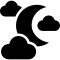
\includegraphics{./images/Nacht}

\end{column}

\begin{column}{0.34\textwidth}

~

\end{column}

\begin{column}{0.33\textwidth}

\textbf{Nacht} \citep{Nacht} {[}\emph{Noc}{]} Ćwierć wieku po Het is een nacht Guus Meeuwis wykonał ``Nacht'' wraz z raperem Kraantje Pappie. Posłuchajcie sami.

\end{column}

\vfill

\begin{column}{0.48\textwidth}

\emph{Het is een nacht}\\
\emph{Die je normaal alleen in films ziet}\\
\emph{Het is een nacht}\\
\emph{Die wordt bezongen in het mooiste lied}\\
\emph{Het is een nacht}\\
\emph{Waarvan ik dacht dat ik hem nooit beleven zou}\\
\emph{Maar vannacht beleef ik hem met jou oh oh}

\end{column}

\begin{column}{0.04\textwidth}

~

\end{column}

\begin{column}{0.48\textwidth}

\emph{To jest taka noc}\\
\emph{Którą widzisz zwykle tylko w filmach}\\
\emph{To jest taka noc}\\
\emph{O której mówi najpiękniejsza piosenka}\\
\emph{To jest taka noc}\\
\emph{O której myślałem, że jej nigdy nie przeżyję}\\
\emph{A którą dziś przeżywam z tobą Ooo}

\end{column}

\vfill

\begin{column}{0.48\textwidth}

Op de grond ligt Châteauneuf-du-Pape\\
De radio zacht, rond middernacht\\
Ik hoor Suus en Freek, een blauwe dag\\
En ik kijk hoe je slaapt, ik hou je vast\\
Want ik weet dat het niet lang meer duurt voor jij gaat\\
Ik snap dat jij me niet te dichtbij laat\\
En je weer vrijmaakt en je op tijd staat\\
Je twijfelt aan of ik wel echt meen wat ik heb gezegd\\
En of ik nog steeds wel de echte ben\\
En of ik niet ren naar 050 en je niet meer ken als een slechte vent\\
Maar vannacht is dat allemaal niet de case\\
Voor nu is het nog nooit zo mooi geweest\\
Jij en ik, the road can wait\\
En ben ik voor eerst opeens compleet

\end{column}

\begin{column}{0.04\textwidth}

~

\end{column}

\begin{column}{0.48\textwidth}

Na ziemi leży Châteauneuf-du-Pape\\
Radio cicho gra, jest koło północy\\
Słyszę Suus i Freek, jakiś niebieski dzień\\
Patrzę jak śpisz, przytulam cię\\
Bo wiem, że to nie potrwa już długo zanim wyjdziesz\\
Rozumiem, że nie pozwolisz mi się zbliżyć\\
En je weer vrijmaakt en je op tijd staat\\
Wątpisz, czy naprawdę mam na myśli to, co powiedziałem\\
I czy nadal jestem prawdziwy\\
I czy nie biegnę na 50 i już cię nie znam jak jakiś zły facet\\
Ale dziś w nocy to w ogóle nie o to chodzi\\
Jeszcze nigdy nie było tak pięknie\\
Ty i ja, droga może poczekać\\
Nagle po raz pierwszy jestem spełniony

\end{column}

\vfill

\begin{column}{0.48\textwidth}

\emph{Als het komt, zou ik steeds met je zijn}\\
\emph{En als je wennen moet, begrijp ik baby, neem je de tijd}\\
\emph{Hier leven we voor, plus cash en baguettes}\\
\emph{En deze nacht heeft alles wat ik zocht op deze plek}

\end{column}

\begin{column}{0.04\textwidth}

~

\end{column}

\begin{column}{0.48\textwidth}

\emph{Gdyby tak się stało, zawsze byłbym z tobą}\\
\emph{A jeśli musisz się zastanowić, rozumiem to baby, nie spiesz się}\\
\emph{Po to żyjemy, plus kasa i bagietki}\\
\emph{I ta noc ma wszystko, co szukałem w tym miejscu}

\end{column}

\vfill

\begin{column}{0.48\textwidth}

Hey schat, ik zou m'n kleine teen geven voor nog één nacht\\
Het is natuurlijk geen wonder dat ik je\\
Donderdag al bijzonder zag in het dons gepakt heb\\
En onze nacht werd er één als\\
Die van Leo en Kate was\\
We on top of the world, ben volledig gebrainwashed\\
But I like it, yeah, jij showt wat life is\\
En ja, je life is er een als Kylie's\\
Maar net iets ronder en iets gezonder\\
Dat is precies hoe mijn vibe is, yeah\\
Jij bent de nicest\\
Bel de Bel, boy, bestel champagne\\
Fuck the prices, je rolt met Crane

\end{column}

\begin{column}{0.04\textwidth}

~

\end{column}

\begin{column}{0.48\textwidth}

Hej kochanie, oddałbym mój mały palec u nogi za jeszcze jedną noc\\
Oczywiście to nic dziwnego, że ja ciebie\\
Donderdag al bijzonder zag in het dons gepakt heb\\
A nasza noc stała się taką jedną,\\
Jaka należała do Leo i Kate\\
Jesteśmy na szczycie świata, mam kompletnie wyprany mózg\\
Ale lubię to, tak, pokazujesz, czym jest życie\\
I tak, twoje życie jest takie jak życie Kylie\\
Ale nieco bardziej zaokrąglone i nieco zdrowsze\\
Dokładnie taki jest mój klimat, tak\\
Jesteś najmilsza\\
Bel de Bel, chłopie, zamówmy szampana\\
Pieprzyć ceny, ty kręcisz z Crane

\end{column}

\vfill

\begin{column}{0.48\textwidth}

Maar vannacht beleef ik 'm met jou, oh\\
Ja ik hou alleen nog maar van jou\\
Ja ik hou alleen nog maar van jou

\end{column}

\begin{column}{0.04\textwidth}

~

\end{column}

\begin{column}{0.48\textwidth}

Ale dziś przeżywam ją z tobą Ooo\\
I kocham tylko wyłącznie ciebie\\
I kocham tylko wyłącznie ciebie

\end{column}

\vfill

\begin{quote}
\textbf{Châteauneuf-du-Pape} fr. cenione wino\\
\textbf{Suus en Freek} duet wykonujący Blauwe Dag \ref{Blauwe-dag}\\
\textbf{Leo en Kate} para z filmu Titanic\\
\textbf{Kylie} amerykańska celebrytka\\
\textbf{Bel de Bel} właść. fr. La Belle des belles\\
\textbf{Crane} od Kraantje, wykonawcy piosenki
\end{quote}

\hypertarget{Het-is-een-nacht}{%
\section{\texorpdfstring{Het is een nacht, \emph{Guus Meeuwis}}{Het is een nacht, Guus Meeuwis}}\label{Het-is-een-nacht}}

\begin{column}{0.33\textwidth}

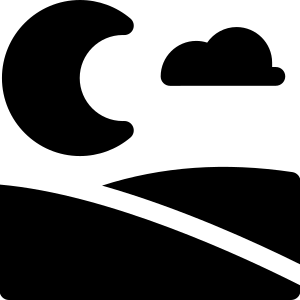
\includegraphics{./images/Het-is-een-nacht}

\end{column}

\begin{column}{0.34\textwidth}

~

\end{column}

\begin{column}{0.33\textwidth}

\textbf{Het is een nacht} \citep{Het-is-een-nacht} {[}\emph{To jest taka noc}{]} powstała po romantycznym weekendzie, jaki spędził autor ze swoją dziewczyną Valérie Gregoire w Brugii.

\end{column}

\vfill

\begin{column}{0.48\textwidth}

Je vraagt of ik zin heb in een sigaret\\
Het is twee uur 's nachts\\
We liggen op bed\\
In een hotel in een stad\\
Waar niemand ons hoort\\
Waar niemand ons kent\\
En niemand ons stoort\\
Op de vloer ligt een lege fles wijn\\
En kledingstukken die van jou of mij kunnen zijn\\
Een schemering de radio zacht\\
En deze nacht heeft alles\\
Wat ik van een nacht verwacht

\end{column}

\begin{column}{0.04\textwidth}

~

\end{column}

\begin{column}{0.48\textwidth}

Pytasz, czy mam ochotę na papierosa\\
Jest druga w nocy\\
Jesteśmy w łóżku\\
W hotelu, w mieście\\
Gdzie nikt nas nie słyszy\\
Gdzie nikt nas nie zna\\
I nikt nam nie przeszkadza\\
Na podłodze leży pusta butelka po winie\\
I ubrania, które mogą być twoje lub moje\\
Półmrok, radio cicho gra\\
I ta noc ma wszystko\\
Czego oczekuję od nocy

\end{column}

\vfill

\begin{column}{0.48\textwidth}

\emph{Het is een nacht}\\
\emph{Die je normaal alleen in films ziet}\\
\emph{Het is een nacht}\\
\emph{Die wordt bezongen in het mooiste lied}\\
\emph{Het is een nacht}\\
\emph{Waarvan ik dacht dat ik hem nooit beleven zou}\\
\emph{Maar vannacht beleef ik hem met jou ohoh}

\end{column}

\begin{column}{0.04\textwidth}

~

\end{column}

\begin{column}{0.48\textwidth}

\emph{To jest taka noc}\\
\emph{Którą widzisz zwykle tylko w filmach}\\
\emph{To jest taka noc}\\
\emph{O której mówi najpiękniejsza piosenka}\\
\emph{To jest taka noc}\\
\emph{O której myślałem, że jej nigdy nie przeżyję}\\
\emph{A którą dziś przeżywam z tobą Ooo\ldots{}}

\end{column}

\vfill

\begin{column}{0.48\textwidth}

Ik ben nog wakker en ik staar naar het plafond\\
En ik denk aan de dag lang geleden begon\\
Het zomaar er vandoor gaan met jou\\
Niet wetend waar de reis eindigen zou\\
Nu lig ik hier in een wildvreemde stad\\
En heb net de nacht van mijn leven gehad\\
Maar helaas er komt weer licht door de ramen\\
Hoewel voor ons de wereld\\
Vannacht heeft stil gestaan

\end{column}

\begin{column}{0.04\textwidth}

~

\end{column}

\begin{column}{0.48\textwidth}

Nadal nie śpię i wpatruję się w sufit\\
I myślę o tym dniu co zaczął się tak dawno\\
Tak po prostu przemija przy tobie\\
Nie wiedząc, gdzie zakończy się ta podróż\\
Teraz leżę tutaj w zupełnie obcym mieście\\
I właśnie miałem noc swojego życia\\
Ale niestety światło znów wpada przez okna\\
Ale co tam, świat dla nas\\
Zatrzymał się dziś w nocy

\end{column}

\vfill

\begin{column}{0.48\textwidth}

Maar een lied blijft slechts bij woorden\\
Een film is in scene gezet\\
Maar deze nacht met jou\\
Is levensecht

\end{column}

\begin{column}{0.04\textwidth}

~

\end{column}

\begin{column}{0.48\textwidth}

Ale piosenka to tylko słowa\\
Film jest na scenie zagrany\\
Ale dzisiejsza noc z tobą\\
Jest prawdziwa

\end{column}

\vfill

\begin{column}{0.48\textwidth}

En vannacht beleef ik hem met jou ohoh\\
En ik hou alleen nog maar van jou ohoh\\
En ik hou alleen nog maar van jou

\end{column}

\begin{column}{0.04\textwidth}

~

\end{column}

\begin{column}{0.48\textwidth}

I dziś przeżywam ją z tobą Ooo\ldots{}\\
I kocham tylko wyłącznie ciebie Ooo\ldots{}\\
I kocham tylko wyłącznie ciebie

\end{column}

\vfill

\begin{quote}
\textbf{Je bent trouwens eigenlijk wel geweldig.} Nawiasem mówiąc, jesteś naprawdę świetny.\\
\textbf{Als ik niet Pools was, zou ik geen Pools kennen.} Gdybym nie był Polakiem, nie znałbym polskiego.\\
\textbf{Heb ik daarvoor een vergunning nodig?} Czy potrzebuję na to zezwolenie?\\
\textbf{Waar kan ik meer te weten komen over \ldots?} Gdzie mogę dowiedzieć się więcej o\ldots?\\
\textbf{Wanneer \ldots{}} Kiedy \ldots\ldots..?\\
\textbf{Ik heb zin in een borrel.} Mam ochotę na drinka.\\
\textbf{De lijn is bezet. Linia jest zajęta}\\
\textbf{Als ik meer tijd had, zou ik op je wachten.} Gdybym miał/a więcej czasu, poczekałbym na ciebie.\\
\textbf{Je moeder kan echt lekker koken.} Twoja mama naprawdę potrafi dobrze gotować.\\
\textbf{Dat is veel, he?} To dużo, prawda?\\
\textbf{Wanneer moet ik terugkomen?} Kiedy muszę wrócić?\\
\textbf{Zullen wij naar de duinen gaan?} Może pójdziemy na wydmy?
\end{quote}

\hypertarget{Blauwe-dag}{%
\section{\texorpdfstring{Blauwe dag, \emph{Suzan \& Freek}}{Blauwe dag, Suzan \& Freek}}\label{Blauwe-dag}}

\begin{column}{0.33\textwidth}

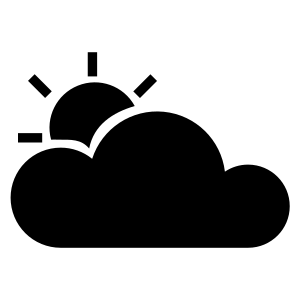
\includegraphics{./images/Blauwe-dag}

\end{column}

\begin{column}{0.34\textwidth}

~

\end{column}

\begin{column}{0.33\textwidth}

\textbf{Blauwe dag} \citep{Blauwe-dag} {[}\emph{Gorszy dzień}{]} powstała po romantycznym weekendzie, jaki spędził autor ze swoją dziewczyną Valérie Gregoire w Brugii.

\end{column}

\vfill

\begin{column}{0.48\textwidth}

Weet je nog dat jij me zei dat wij nooit zouden vluchten als een van ons\\
Loopt door de regen en nooit meer kijkt naar hoe het leven is in de zon\\
Weet je nog dat jij me zei dat jij d'r altijd bent als ik je nodig heb\\
Nee, ik ben het niet vergeten, nee\\
Wat jij me ooit hebt gezegd\\
Want ik zie dat jij het moeilijk hebt en niet meer lachen kan zoals je vroeger deed\\
En nauwelijks in de gaten hebt dat je anders loopt dan dat je deed voorheen\\
Weet je nog dat jij me zei dat jij d'r altijd bent als ik je nodig heb\\
Nee, ik ben het niet vergeten, nee\\
Wat jij me ooit hebt gezegd

\end{column}

\begin{column}{0.04\textwidth}

~

\end{column}

\begin{column}{0.48\textwidth}

Czy pamiętasz, jak mi powiedziałaś, że nigdy nie moglibyśmy uciec, gdyby któreś z nas\\
Szło w deszczu i nie widziało więcej jakie jest życie w słońcu\\
Pamiętasz, jak mi powiedziałeś, że tam zawsze jesteś, kiedy ja cię potrzebuję\\
Nie, ja tego nie zapominałam, nie\\
Co mi kiedyś powiedziałeś\\
Ponieważ widzę, że masz trudności i nie możesz się uśmiechać tak jak kiedyś\\
I prawie nie zauważasz, że chodzisz inaczej niż kiedyś\\
Czy pamiętasz, jak mi powiedziałaś, że tam zawsze jesteś, kiedy ja cię potrzebuję\\
Nie, ja tego nie zapomniałam, nie\\
Co mi kiedyś powiedziałeś

\end{column}

\vfill

\begin{column}{0.48\textwidth}

\emph{Blauwe dag, als het dondert}\\
\emph{En valt de hemel naar beneden, ben ik hier bij jou alleen}\\
\emph{Blauwe dag, een seconde}\\
\emph{Laten we dansen tot de morgen en de lucht weer opengaat}\\
\emph{Fiets met jou mee door heel de stad}\\
\emph{Als jij dat wil, nou, dan doe ik dat}\\
\emph{Ik ben hier op je blauwe dag}\\
\emph{Blauwe dag, een seconde}\\
\emph{Laten we dansen tot de morgen en de lucht weer opengaat}

\end{column}

\begin{column}{0.04\textwidth}

~

\end{column}

\begin{column}{0.48\textwidth}

\emph{Gorszy dzień, kiedy grzmi}\\
\emph{I niebo spada w dół, jestem tu sam przy tobie}\\
\emph{Gorszy dzień, jedna sekunda}\\
\emph{Tańczmy do rana i niebo znów się otwiera}\\
\emph{Jechać z tobą na rowerze przez całe miasto}\\
\emph{Jeśli tego chcesz, teraz, to ja to zrobię}\\
\emph{Jestem tu w twój gorszy dzień}\\
\emph{Gorszy dzień, jedna sekunda}\\
\emph{Przetańczmy tę noc, a niebo znów się przejaśni}

\end{column}

\vfill

\begin{column}{0.48\textwidth}

Weet je nog dat jij me zei dat jij d'r altijd bent wanneer ik ergens val\\
Nu lig ik zelf op de grond en ben ik diegene zonder licht in een donker dal\\
Ik ging van de top van de wereld naar de plek waar ik niemand ken\\
Nee, ik ben het niet vergeten, nee\\
Wat jij me ooit hebt gezegd\\
Blauwe dag, als het dondert\\
En valt de hemel naar beneden, ben ik hier bij jou alleen

\end{column}

\begin{column}{0.04\textwidth}

~

\end{column}

\begin{column}{0.48\textwidth}

Pamiętasz, kiedy powiedziałeś mi, że zawsze tam jesteś, kiedy gdzieś upadam\\
Nu lig ik zelf op de grond en ben ik diegene zonder licht in een donker dal\\
Ik ging van de top van de wereld naar de plek waar ik niemand ken\\
Nee, ik ben het niet vergeten, nee\\
Wat jij me ooit hebt gezegd\\
Blauwe dag, als het dondert\\
En valt de hemel naar beneden, ben ik hier bij jou alleen

\end{column}

\vfill

\begin{column}{0.48\textwidth}

Fiets met jou mee door heel de stad\\
Als jij dat wil, nou, dan doe ik dat\\
Ik ben hier op je blauwe dag\\
Blauwe dag, een seconde\\
Laten we dansen tot de morgen en de lucht weer opengaat

\end{column}

\begin{column}{0.04\textwidth}

~

\end{column}

\begin{column}{0.48\textwidth}

Fiets met jou mee door heel de stad\\
Als jij dat wil, nou, dan doe ik dat\\
Ik ben hier op je blauwe dag\\
Blauwe dag, een seconde\\
Laten we dansen tot de morgen en de lucht weer opengaat

\end{column}

\vfill

\begin{quote}
\textbf{De lucht wordt donker.} Niebo robi się ciemne.\\
\textbf{De lucht klaarde op.} Niebo się przejaśniło.\\
\textbf{De hemel is blauw} Niebo jest niebieskie.\\
\textbf{Zijn ziel was in het hemel} Jego dusza była w niebie.\\
\textbf{Ik voel me blauw.} Jestem przygnębiony.\\
\textbf{Weet je nog?} Czy pamiętasz?\\
\textbf{Laten we haar alleen laten.} Zostawmy ją w spokoju.\\
\textbf{Ik denk dat wij goede vrienden zouden kunnen zijn.} Myślę, że moglibyśmy być dobrymi przyjaciółmi.\\
\textbf{Hij kan nauwelijks lezen.} On ledwo umie czytać.\\
\textbf{Houd deze koffer in de gaten.} Obserwuj tę walizkę.
\end{quote}

\hypertarget{Dromen-zijn-bedrog}{%
\section{\texorpdfstring{Dromen zijn bedrog, \emph{Marco Borsato}}{Dromen zijn bedrog, Marco Borsato}}\label{Dromen-zijn-bedrog}}

\begin{column}{0.33\textwidth}

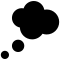
\includegraphics{./images/Dromen-zijn-bedrog}

\end{column}

\begin{column}{0.34\textwidth}

~

\end{column}

\begin{column}{0.33\textwidth}

\textbf{Dromen zijn bedrog} \citep{Dromen-zijn-bedrog} {[}\emph{Sny są ulotne}{]} jest uważana za jeden z najbardziej udanych singli w języku niderlandzkim wszech czasów.

\end{column}

\vfill

\begin{column}{0.48\textwidth}

Steeds als ik je zie lopen dan gaat de hemel een klein beetje open\\
Sterren, je laat ze verbleken met je ogen die altijd stralen\\
Jij kan de zon laten schijnen want je loopt langs en de wolken verdwijnen en als je lacht, lacht heel de wereld mee

\end{column}

\begin{column}{0.04\textwidth}

~

\end{column}

\begin{column}{0.48\textwidth}

Zawsze, kiedy widzę jak idziesz, wtedy odrobinę otwiera się niebo\\
Gwiazdy, sprawiasz że one bledną, swoimi oczami, które cały czas promienieją\\
Możesz pozwolić słońcu świecić, bo gdy przechodzisz chmury znikają a kiedy się śmiejesz, razem śmieje się cały świat

\end{column}

\vfill

\begin{column}{0.48\textwidth}

\emph{De meeste dromen zijn bedrog maar als ik wakker word naast jou dan droom ik nog}\\
\emph{Ik voel je adem en zie je gezicht je bent een droom die naast me ligt}\\
\emph{Je kijkt me aan en rekt je uit een keer in de zoveel tijd komen dromen uit!}

\end{column}

\begin{column}{0.04\textwidth}

~

\end{column}

\begin{column}{0.48\textwidth}

\emph{Najczęściej sny są ulotne, ale kiedy budzę się obok ciebie, wciąż marzę}\\
\emph{Czuję twój oddech i widzę twoją twarz, jesteś snem leżącym obok mnie}\\
\emph{Patrzysz na mnie i się wyciągasz raz na jakiś czas marzenia się spełniają!}

\end{column}

\vfill

\begin{column}{0.48\textwidth}

Jij moet me een ding beloven laat me nog lang in mijn dromen geloven\\
Zelfs als je even niet hier bent blijf in mijn slaap dan bij me\\
En als de zon weer gaat schijnen laat dan dat beeld wat ik heb niet verdwijnen. Als je zou gaan, neem je mijn dromen mee

\end{column}

\begin{column}{0.04\textwidth}

~

\end{column}

\begin{column}{0.48\textwidth}

Musisz mi obiecać jedno, pozwól mi jeszcze długo wierzyć w moje marzenia\\
Nawet jeśli cię chwilę tutaj nie ma, zostań ze mną kiedy śpię\\
A kiedy znów zaświeci słońce, nie pozwól fantazji którą mam zniknąć. Gdybyś szła, zabierz ze sobą moje marzenia

\end{column}

\vfill

\begin{quote}
\textbf{Dromen zijn bedrog.} Sen mara, Bóg wiara. {[}prov. za Czochralski{]}\\
\textbf{Met een klein beetje geluk.} Przy odrobinie szczęścia.\\
\textbf{De deur gaat niet open, hij klemt.} Drzwi się nie otwierają, są zablokowane.\\
\textbf{Kom met me mee.} Chodź razem ze mną.\\
\textbf{Als ik vragen mag.} Jeśli wolno spytać.\\
\textbf{Ik reik mijn hand naar je uit.} Wyciągam rękę do ciebie.\\
\textbf{De narcissen kwamen uit.} Wypuściły żonkile.\\
\textbf{Een keer in de zoveel tijd.} Raz na jakiś czas.\\
\textbf{Mag ik even binnenkomen?} Czy mogę na chwilę wejść?\\
\textbf{Ik blijf in slaap vallen.} Ciągle zasypiam.\\
\textbf{Wat heb je vannacht gedroomd?} Co ci się śniło dzisiaj w nocy?\\
\textbf{Waar droom je over?} O czym marzysz?
\end{quote}

\hypertarget{Ik-kan-het-niet-alleen}{%
\section{\texorpdfstring{Ik kan het niet alleen, \emph{De Dijk}}{Ik kan het niet alleen, De Dijk}}\label{Ik-kan-het-niet-alleen}}

\begin{column}{0.33\textwidth}

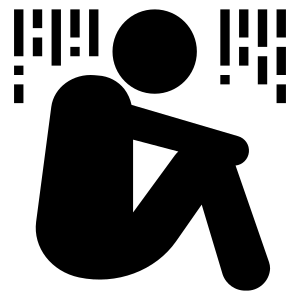
\includegraphics{./images/Ik-kan-het-niet-alleen}

\end{column}

\begin{column}{0.34\textwidth}

~

\end{column}

\begin{column}{0.33\textwidth}

\textbf{Ik kan het niet alleen} \citep{Ik-kan-het-niet-alleen} {[}\emph{Nie mogę tego zrobić sam}{]} to jedna z najbardziej znanych piosenek De Dijk do dziś odtwarzana przez wiele stacji radiowych w Holandii..

\end{column}

\vfill

\begin{column}{0.48\textwidth}

Elke morgen, elke middag\\
Elke avond, iedere nacht\\
Stel dat ik er wel maar jij er niet was\\
Dan was morgen morgen waarschijnlijk weer zo'n dag\\
En ik kan 't niet\\
ik kan 't niet\\
ik kan er niet omheen\\
k-k-kan 't niet\\
ik kan 't niet alleen\\
Natte ramen, kale muren\\
Lege flessen op de gang\\
Lange tanden, late uren\\
Weinig zon en veel behang\\
Ik heb het geprobeerd gedaan wat ik kan\\
maar alles gaat verkeerd\\
Ik ben ook maar een man\\
En ik kan het niet alleen

\end{column}

\begin{column}{0.04\textwidth}

~

\end{column}

\begin{column}{0.48\textwidth}

Co rano, co południe\\
Co wieczór, każdej nocy\\
Stel dat ik er wel maar jij er niet was\\
Jutro prawdopodobnie znowu taki dzień\\
En ik kan 't niet\\
ik kan 't niet\\
ik kan er niet omheen\\
k-k-kan 't niet\\
ik kan 't niet alleen\\
Mokre okna, gołe ściany\\
Puste butelki na korytarzu\\
Brak apetytu Późne godziny\\
Niewiele słońca i wiele tapet\\
Próbowałem zrobić, co mogłem\\
ale wszystko idzie źle\\
Jestem tylko człowiekiem\\
I nie mogę tego zrobić sam

\end{column}

\vfill

\begin{quote}
\textbf{Hij eet met lange tanden.} On je niechętnie.\\
\textbf{Beter laat dan nooit.} Lepiej późno niż wcale.\\
\textbf{We kunnen er niet omheen dat \ldots{}} Nie możemy omijać faktu, że \ldots{}
\end{quote}

\hypertarget{O-o-Den-Haag}{%
\section{\texorpdfstring{O, o, Den Haag, \emph{Harry Klorkestein}}{O, o, Den Haag, Harry Klorkestein}}\label{O-o-Den-Haag}}

\begin{column}{0.33\textwidth}

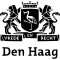
\includegraphics{./images/O-o-Den-Haag}

\end{column}

\begin{column}{0.34\textwidth}

~

\end{column}

\begin{column}{0.33\textwidth}

\textbf{O, o, Den Haag} \citep{O-o-Den-Haag} {[}\emph{Oj, oj, Haga}{]} to piosenka uznawana za nieoficjalny hymn Hagi. Nazwa wykonawcy to anagram nazwy prawdziwego zespołu Klein Orkest.

\end{column}

\vfill

\begin{column}{0.48\textwidth}

Ik zou best nog wel een keertje net als vroeger in Moerwijk willen wonen\\
Na het eten een partijtje voetbal in de tuin, de ouders langs de lijn\\
In december met de hele buurt op jacht om kerstbomen te rausen\\
Op oudejaarsavond fikkie stoken, vooral die autobanden rookten fijn\\
Ik zou best nog wel een keertje met die ouwe naar ADO willen kijken\\
In het Zuiderpark, de lange zij, een warme worst, supporters om je heen\\
Lekker kankeren op Theo van den Burch en die lange van Vianen\\
Want bij elke lage bal dan dook die eikel er steevast overheen\\
O, o, Den Haag, mooie stad achter de duinen\\
De Schilderswijk, de Lange Poten en het Plein\\
O, o, Den Haag, ik zou met niemand willen ruilen\\
Meteen gaan huilen, als ik geen Hagenees zou zijn\\
Ik zou best nog wel een keertje net als vroeger een nachie willen stappen\\
Op mijn Puch een wijffie halen en daarna dansen in de Marathon\\
Na afloop op het Rijswijkseplein een harinkie gaan happen\\
De dag erna een kater dus naar Scheveningen, lekker bakken in de zon\\
Ik zou best nog wel een keertje \ldots{} ach, wat leg ik toch te dromen\\
Want Den Haag is door de jaren zo veranderd, voor mij toch veel te vlug\\
Dat Nieuw Babylon moest dat er trouwens eigenlijk nou wel zo nodig komen?\\
Zo komt die ooievaar op de Vijverberg dus never-nooit meer terug

\end{column}

\begin{column}{0.04\textwidth}

~

\end{column}

\begin{column}{0.48\textwidth}

Bardzo chciałbym raz jeszcze, tak jak kiedyś, na Moerwijku zamieszkać\\
Po obiedzie przyciąć w nogę w ogrodzie, rodzice wzdłuż linii\\
A w grudniu z cała okolica na polowanie co by kilka choinek przyciągnąć\\
W Sylwestra rozniecać pożary, opony dymiły się szczególnie dobrze\\
Bardzo chciałbym raz jeszcze ze starszym na ADO popatrzeć\\
W Zuiderparku, długi bok, ciepła kiełbaska, kibice wokół ciebie\\
Cudne wyzwiska za Theo van den Burch i tym wysokim van Vianen\\
Ponieważ z każdą niska piłka, ten żołądź zawsze przelatywał nad nią\\
O, o, Haga, piękne miasto za wydmami\\
Schilderswijk, Lange Poten no i Plein\\
O, o, Haga, nie chciałbym się z nikim zamienić\\
Płakałbym od razu, gdybym nie był Hażaninem\\
Bardzo chciałbym raz jeszcze, tak jak kiedyś wyjść w noc\\
Zgarnąć laskę na mojego Pucha i potem tańczyć w Marathonie\\
Po wszystkim na Rijswijkseplein pójść śledzika przekąsić\\
Następnego dnia kac, wiec na Scheveningen cudownie smażyć się w słońcu\\
Bardzo chciałbym raz jeszcze \ldots{} ach, o czym ja śnię\\
Ponieważ Haga przez te lata bardzo się zmieniła, jak dla mnie to zbyt szybko\\
Czy ten Nieuw Babylon musiał, tak miedzy nami, się tam pojawić?\\
Wiec nie pojawi się już nigdy więcej bocian na Vijverbergu

\end{column}

\vfill

\begin{quote}
\textbf{Ik heb zin in een borrel.} Mam ochotę na drinka.\\
\textbf{Nog een keer!} Jeszcze raz!\\
\textbf{Je bent trouwens eigenlijk wel geweldig.} Nawiasem mówiąc, jesteś naprawdę świetny.\\
\textbf{Als ik niet Pools was, zou ik geen Pools kennen.} Gdybym nie był Polakiem, nie znałbym polskiego.\\
\textbf{Heb ik daarvoor een vergunning nodig?} Czy potrzebuję na to zezwolenie?\\
\textbf{Waar kan ik meer te weten komen over \ldots?} Gdzie mogę dowiedzieć się więcej o\ldots?\\
\textbf{Dat is veel, he?} To dużo, co?\\
\textbf{Wanneer moet ik terugkomen?} Kiedy muszę wrócić?\\
\textbf{Zullen wij naar de duinen gaan?} Może pójdziemy na wydmy?\\
\textbf{De lijn is bezet.} Linia jest zajęta\\
\textbf{Als ik meer tijd had, zou ik op je wachten.} Gdybym miał/a więcej czasu, poczekałbym na ciebie.\\
\textbf{Je moeder kan echt lekker koken.} Twoja mama naprawdę potrafi dobrze gotować.
\end{quote}

\hypertarget{Avond}{%
\section{\texorpdfstring{Avond, \emph{Boudewijn de Groot}}{Avond, Boudewijn de Groot}}\label{Avond}}

\begin{column}{0.33\textwidth}

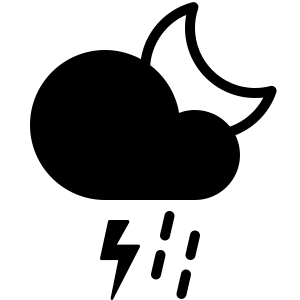
\includegraphics{./images/Avond}

\end{column}

\begin{column}{0.34\textwidth}

~

\end{column}

\begin{column}{0.33\textwidth}

\textbf{Avond} \citep{Avond} {[}\emph{Wieczór}{]} to piosenka uznawana przez Holendrów za najlepszą niderlandzkojęzyczną piosenkę wszechczasóW.

\end{column}

\vfill

\begin{column}{0.48\textwidth}

Nu hoef je nooit je jas meer aan te trekken\\
En te hopen dat je licht het doet\\
Laat buiten de stormwind nu maar razen in het donker\\
Want binnen is het warm en licht en goed\\
Hand in hand naar buiten kijkend waar de regen valt\\
Ik zie het vuur van hoop en twijfel in je ogen\\
En ik ken je diepste angst

\end{column}

\begin{column}{0.04\textwidth}

~

\end{column}

\begin{column}{0.48\textwidth}

Już nie musisz więcej zakładać kurtki\\
I się martwić, czy zapalą światła\\
Niech na dworze w ciemności szaleje wiatr\\
Bo w środku jest ciepło i widno i dobrze\\
Patrząc na dwór, gdzie pada deszcz trzymam cię za rękę\\
W twoich oczach widzę ogień nadziei i zwątpień\\
I znam twój najgłębszy lęk

\end{column}

\vfill

\begin{column}{0.48\textwidth}

\emph{Want je kunt niets zeker weten en alles gaat voorbij}\\
\emph{Maar ik geloof, ik geloof, ik geloof, ik geloof, ik geloof in jou en mij}

\end{column}

\begin{column}{0.04\textwidth}

~

\end{column}

\begin{column}{0.48\textwidth}

\emph{Bo niczego nie możesz być pewna, a wszystko przemija}\\
\emph{Ale wierzę, wierzę, wierzę, wierzę, wierzę w ciebie i we mnie}

\end{column}

\vfill

\begin{column}{0.48\textwidth}

En als je 's morgens opstaat ben ik bij je\\
En misschien heb ik al thee gezet\\
En als de zon schijnt buiten gaan we lopen door de duinen\\
En als het regent gaan we t'rug in bed\\
Uren langzaam wakker worden, zwevend door de tijd\\
Ik zie het licht door de gordijnen\\
En ik weet, t'verleden geeft geen zekerheid

\end{column}

\begin{column}{0.04\textwidth}

~

\end{column}

\begin{column}{0.48\textwidth}

A kiedy wstaniesz rano, to ja będę przy tobie\\
I może herbata już będzie zrobiona\\
I jeśli na dworze będzie słonecznie, to pójdziemy na wydmy\\
A gdyby padało, to wrócimy do łóżka\\
Godziny powoli się budzą unosząc się w czasie\\
Widzę światło przez zasłony\\
I wiem, że przeszłość nie daje pewności

\end{column}

\vfill

\begin{column}{0.48\textwidth}

Ik doe de lichten uit en de kamer wordt nu donker\\
Een straatlantaarn buiten geeft wat licht\\
En de dingen in de kamer worden vrienden die gaan slapen\\
De stoelen staan te wachten op 't ontbijt\\
En morgen wordt ik wakker met de geur van brood en honing\\
De glans van gouden zonlicht in je haar\\
En de dingen in de kamer, ik zeg ze welterusten\\
Vanavond gaan we slapen en morgen zien we wel\\
Maar de dingen in de kamer zouden levenloze dingen zijn\\
Zonder jou

\end{column}

\begin{column}{0.04\textwidth}

~

\end{column}

\begin{column}{0.48\textwidth}

Gaszę światło i teraz w pokoju robi się ciemniej\\
Latarnia na ulicy daje nieco światła\\
A rzeczy w pokoju stają się przyjaciółmi, którzy idą spać\\
Krzesła oczekują na śniadanie\\
A jutro obudzę się z zapachem chleba i miodu\\
Błysk złotych promieni słońca w twoich włosach\\
A rzeczą w pokoju, mówię dobranoc\\
Dzisiaj pójdziemy spać i zobaczymy się znowu jutro\\
Ale rzeczy w pokoju byłyby martwe\\
Bez ciebie

\end{column}

\vfill

\begin{quote}
\textbf{Doe het licht maar uit.} Po prostu wyłącz światło.\\
\textbf{Ik wil je nooit meer zien.} Nie chcę cię nigdy więcej widzieć.\\
\textbf{Ze liepen hand in hand.} Szli trzymając się za ręce.\\
\textbf{Die jongen toonde geen angst.} Ten chłopiec nie okazywał strachu.\\
\textbf{Het is te hopen dat \ldots{}} Należy mieć nadzieją, że \ldots{}\\
\textbf{De vlam zweeft vaak net boven het hout.} Płomień unosi się często tuż nad drewnem.\\
\textbf{Ga Maria wakker maken.} Idź obudź Marię\\
\textbf{Ik sta op het punt uit te gaan.} Zaraz wychodzę.\\
\textbf{De geur van lelies vulde de kamer.} Zapach lilii wypełnił pokój.\\
\textbf{De glans wordt gemeten volgens ISO 2813.} Połysk mierzy się zgodnie z ISO 2813.\\
\textbf{Ik zie je wel bij de auto.} Do zobaczenia w aucie.
\end{quote}

\hypertarget{lata-1980---1989}{%
\chapter{Lata 1980 - 1989}\label{lata-1980---1989}}

Miejsce na rozdział

\hypertarget{lata-1990---1999}{%
\chapter{Lata 1990 - 1999}\label{lata-1990---1999}}

Miejsce na rozdział

\hypertarget{lata-2000---2009}{%
\chapter{Lata 2000 - 2009}\label{lata-2000---2009}}

Miejsce na rozdział

\hypertarget{lata-2010---2019}{%
\chapter{Lata 2010 - 2019}\label{lata-2010---2019}}

Miejsce na rodział

  \bibliography{songs.bib}

\end{document}
